\chapter{Évolution Différentielle sur les circuits simple et double diodes}

\section{Introduction}
Maintenant que nous avons abordé les modèles à diodes et l'Évolution Différentielle indépendemment l'un de l'autre, dans ce chapitre nous allons appliquer l'ED \nomenclature{ED}{Évolution Differentielle (\textit{Differential Evolution})} sur les modèles pour estimer les valeurs des paramètres en utilisant les données expérimentales standards de la littérature. En ce qui concerne l'implémentation pratique de cette technique, on utilise le langage de programmation \textit{Python}. On fait appel a quelques bibliothèques scientifiques de Python pour fournir les outils mathématiques requis par la méthode. A partir d'ici nous allons fournir des petits extraits de code pertinents à la discussion qui montrent la manière d'implémenter les étapes de la méthode. Pour des raisons de clarté ce ne sont pas des extraits complètement fidèles au code utilisé en réalité. Le code complet et non modifié est disponible comme annexe à la fin de ce document. 

\section{Fonction W de Lambert}
Les méthodes évolutionnaires dépendent d'une fonction objectif qu'il faut minimiser, pour sélectionner les meilleures solutions dans une population. Dans notre cas, la fonction objectif est la \textit{RMSE} \nomenclature{RMSE}{Racine de l'erreur quadratique moyenne (\textit{Root Mean Squared Error})} et elle quantifie la différence entre la courbe caractéristique du modèle et les données expérimentales. Cependant, chaque fois qu'un vecteur solution $\vec{V}$ (formules \ref{eq:vsol}) est généré, il faut pouvoir recréer la courbe I-V associée pour permettre à la fonction objectif de calculer la RMSE.
\begin{equation}
  \label{eq:vsol}
  \vec{V}_{\text{simple diode}} = 
  \begin{bmatrix}
    R_s\\
    R_{p}\\
    a\\
    I_0\\
    I_{PV}
  \end{bmatrix},
  \quad
  \vec{V}_{\text{double diode}} = 
  \begin{bmatrix}
    R_s\\
    R_{p}\\
    a_1\\
    a_2\\
    I_{01}\\
    I_{02}\\
    I_{PV}
  \end{bmatrix}
\end{equation}
On pourrait implémenter la fonction objectif en code de la manière suivante:
\begin{python}
# Cette fonction prend un vecteur solution et les points IV experimentaux comme arguments
def objf(vecteur, exp_v, exp_i):
    # Penalisons le vecteur si les valeurs sont non-physiques
    rs, rp = vecteur[0], vecteur[1]
    if rs < 0 or rp < 0:
        return 100 # Valeur fitness large
    ical = i_from_vect(vector, exp_vol) # Une fonction donnant la caracteristique IV de "vector"
    erreur = ical - exp_i
    return np.sqrt(np.mean(erreur ** 2)) # RMSE  
\end{python}

Les équations de modèles simple et double diode (équations \ref{eq:single}, \ref{eq:doublediode}, respectivement) sont transcendantes, il est donc impossible d'extraire directement le courant à partir de la tension et des paramètres (Le courant $I$ figure simultanément dans le premier membre et dans l'exponentiel du second). Ainsi, il n'est pas trivial de remplir la fonction de \pyth{i_from_vect(vector, exp_vol)}. Plusieurs méthodes on été utilisées initialement avec des approches d'approximation analytique ou itérative \cite{Shur1991,AbuelmaAtti1992,Datta1992}. Ces méthodes sont approximatives mais permettent de trouver la solution explicitement avec des fonctions élémentaires (Développement Taylor par exemple). Dans notre cas, on fait recours à la méthode de Jain et Kapoor (2004) \cite{Jain2004, Lun2015} qui utilisent la fonction W de Lambert pour une solution analytique exacte de ces équations.

\subsection{Définition}
La "\textit{fonction W}" de Lambert est définie comme l'inverse de la fonction $w \rightarrow f(w) =  w e^w$, où $w = W_k(z)\ |\ z \in \mathbb{C}$. La fonction $f$ n'étant pas surjective, la fonction $W_k(z)$ est donc \textit{multivaluée} et comprends plusieurs branches indexées par $k$ ($W_0$ est choisie comme branche principale). Si $x \in \mathbb{R}$, donc pour $-1/e \leq x < 0$, il existe deux valeurs réelles possible de $W(x)$ (figure \ref{fig:lambertw}).

\begin{figure} 
  \begin{center}
    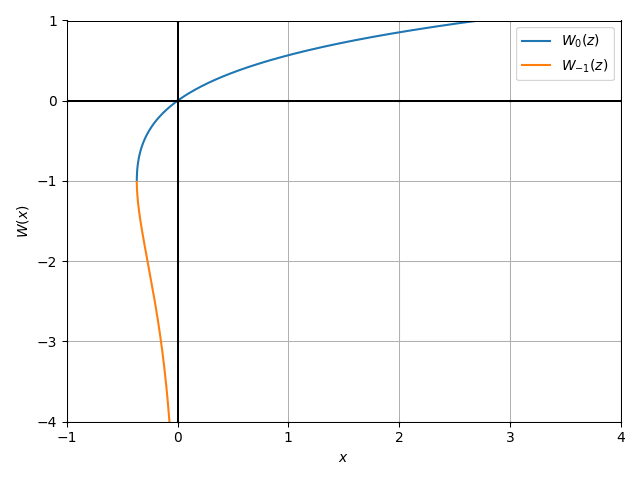
\includegraphics[width=.6\textwidth]{resources/lambertw.png}
    \caption{Les deux branches réelles de $W(x)$ lorsque $x$ est réel}
    \label{fig:lambertw}
  \end{center}
\end{figure}

\subsection{Évaluation de la fonction $W$}

Le fait qu'il n'existe pas de fonctions mathématiques élémentaires donnant explicitement $W(z)$ est remédié par l'existence de plusieurs \textit{algorithmes de recherche des zéros} permettant le calcul de les valeurs de n'importe quelle branche de la fonction $W$. Dans notre cas spécifique, la bibliothèque scientifique \textit{scipy} de Python fournit une fonction W implémentée par l'itération de Halley qui est un exemple d'une méthode de classe "Householder". La méthode de Halley a été appliquée à la fonction $W$  par Corless et al. \cite{Corless1996} donnant:
\begin{equation}
  \label{eq:halley}
  w_{j+1} = w_j - \frac{w_j e^{w_j} - z}{e^{w_j}(w_j + 1) - \frac{(w_j + 2)(w_j e^{w_j} - z)}{2w_j + 2}}
\end{equation}

Un exemple basique de l'utilisation de cette méthode en Python est le suivant:

\begin{python}[basicstyle=\tiny]
import numpy as np 
from scipy.special import lambertw # scipy fournit la fonction W

z = np.linspace(-1/np.e, 3, 1000) # evaluons W entre -1/e et 3
w0 = lambertw(z, 0) # choisir la branche principale
\end{python}

\subsection{Résolution de modèles simple et double diode par la fonction W}
De la définition de la fonction W, la solution d'une équation $xe^x = a$ est $x = W(a)$. En effectuent des manipulations algébriques élémentaires sur le modèle simple diode (equation \ref{eq:single}), Jain et Kapoor ont montré que l'expression explicite du courant en fonction des paramètres et de la tension est:
\begin{equation}
  \label{eq:lambertwsingle}
  I = \frac{R_{sh}(I_0 + I_{PV}) - V}{R_s + R_{sh}} - \frac{W\left(\frac{R_s I_0 R_{sh}}{a V_{th}(R_s + R_{sh})}e^{\left(\frac{R_{sh}(R_s I_{PV} + R_s I_0 + V)}{a V_{th} (R_s + R_{sh})}\right)}\right)aV_{th}}{R_s}
\end{equation}
On remarque bien que le second membre ne contient nul part un terme de courant $I$. Il faut noter aussi que le terme de la fonction $W$ est sous risque d'un dépassement et de retourner de valeurs infinies. Pour des raisons de stabilité numérique on utilise la notion de \textit{Conductance Shunt}: $C_{sh} = \frac{1}{R_{sh}}$ car cette résistance prend souvent de valeurs $\gg 1$ ce qui entraîne un risque de divergence des calculs. On trouve souvent des valeurs larges de résistance shunt, ce qui explique l'existence dans la littérature de plusieurs modèles utilisant la simplification $R_{sh} = + \infty$. Avec la substitution de la conductance shunt, si $R_{sh}\rightarrow\infty$ alors $C_{sh} \rightarrow 0$ ce qui assure la stabilité du calcul numérique.

Le modèle double diodes (équation \ref{eq:doublediode}) contient un terme exponentiel pour chaque diode. De la même manière que Jain et Kapoor on retrouve explicitement l'expression du courant avec deux termes de la fonction $W$ (equation \ref{eq:lambertwdouble}).
\begin{equation}
  \label{eq:lambertwdouble}
  \begin{split}
    I &= \frac{R_{sh} (I_{01} + I_{02} + I_{PV}) - V}{R_s + R_{sh}}\\ 
    &- \frac{a_1}{2 R_s} W\left( \frac{R_s R_{sh}(I_{01} + I_{02})}{a_1 (R_s + R_{sh})}e^{\left(\frac{R_{sh}(R_s I_{PV} + R_s I_{01} + R_s I_{02} + V)}{a_1 (R_s + R_{sh})}\right)}\right)\\ 
    &- \frac{a_2}{2 R_s} W\left( \frac{R_s R_{sh}(I_{01} + I_{02})}{a_1 (R_s + R_{sh})}e^{\left(\frac{R_{sh}(R_s I_{PV} + R_s I_{01} + R_s I_{02} + V)}{a_2 (R_s + R_{sh})}\right)}\right)
  \end{split}
\end{equation}

\section{Résultats}

\subsection{Configuration de l'Évolution Différentielle}
\nomenclature{$F$}{Facteur de mutation}
\nomenclature{$CR$}{Taux de croisement}
\nomenclature{$N_P$}{Taille de la population}
%\nomenclature{$Gen_{max}$}{Nombre maximal de générations}
\nomenclature{$D$}{Dimensions de l'espace de recherche}
Pour appliquer l'Évolution Différentielle avec succès sur les modèles à diodes, il faut savoir choisir les bonnes valeurs de paramètres de contrôle $CR, F \text{et}\  N_P$. Il n'existe pas de règle stricte mais Storn et Price \cite{Price2005} donnent quelques indications. En ce qui concerne le facteur de mutation $F$, les valeurs $F \geq 1$ ne sont pas fiables et souvent convergent très lentement par rapport aux $F < 1$. Cependant, Zaharie (2002) \cite{Zaharie2002} constate une borne inférieure de $F > 0.4$. Puisque l'opération de \textit{sélection} tend à réduire la diversité dans la population, le rôle de la \textit{mutation} et de balancer cette pression exercée sur la population et tend à augmenter la diversité. Si $F$ est trop petit, l'ED peut converger même avec l'absence de la pression sélective. En ce qui concerne le taux de croisement $CR$, Salomon (1996) \cite{Salomon1996} a démontré les limites d'un $CR$ trop petit et par conséquent Storn et Price recommandent des valeurs de $CR$ proche de $1$. Reste à choisir la taille de la population $N_P$, généralement $10D \leq N_P \leq 20D$ est recommandé mais dans notre cas on optera à $N_P = 100$.

\subsection{Cas 1: Cellule 57-mm de RTC France}

Ce premier cas d'étude concerne la cellule en silicium de RTC France avec un diamètre de 57 mm qui a été très largement étudiée dans la littérature. Sa courbe caractéristique a été mesurée dans des conditions de température $T = \SI{33}{\celsius}$ et irradiance solaire $\SI{1000}{\watt\per\square\meter}$ et comprend 26 points expérimentaux (figure \ref{fig:RTCexp}). Figure \ref{fig:RTCres}.a montre que la caractéristique expérimentale et calculée par l'ED sont graphiquement quasi-identiques. Figure \ref{fig:RTCres}.b montre l'évolution de la moyenne des valeurs de fitness des vecteurs évalués par la fonction objectif dans chaque génération consécutive. On constate que dès la 50\textsuperscript{ème} génération, l'ED a pratiquement déjà convergé.

Le tableau \ref{tab:RTCres} présente une comparaison entre l'ED et d'autre méthodes appliquées à la cellule RTC France. On constate que les valeurs retrouvées par l'ED sont assez proches de celles des autres travaux. En effet, l'ED parvient à une erreur RMSE de \num{7.7692e-04} qui est supérieure aux autres techniques similaire comme les essaims particulaires \cite{Hamid2016}, l'algorithme des colonies d'abeilles artificielles \cite{Oliva2014} et l'ED à trois points \cite{Chin2019}. Les résultats les moins précis sont ceux de la méthode de Newton à moindres carrés \cite{Easwarakhanthan1986}.

\begin{table}
  \caption{Bornes utilisées de l'espace de recherche pour le modèle simple diode}
  \label{tab:singleboundaries}

  \begin{center}
    \begin{tabular*}{.7\textwidth}{l@{\extracolsep{\fill}}cc}
       \hline
       \textbf{Paramètre} & \textbf{Borne inférieure} & \textbf{Borne supérieure}   \\
       \hline
       $R_s$    & 0 & 1 \\
       $R_{sh}$ & 2 & 100 \\
       $a$      & 1 & 2\\
       $I_0$    & \num{1e-07} & \num{1e-04} \\
       $I_{PV}$ & 0 & 10\\
       \hline
    \end{tabular*}
  \end{center}
\end{table}

\begin{figure}
  \begin{center}
    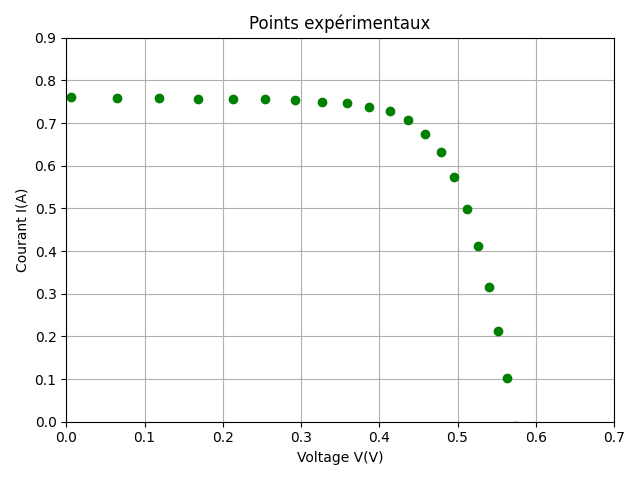
\includegraphics[width=0.6\textwidth]{resources/RTCFrance/exp.png}
    \caption{Données expérimentales de la caractéristique IV de la cellule RTC France mesurées à \SI{33}{\celsius}}
    \label{fig:RTCexp}
  \end{center}
\end{figure}

\begin{figure*}[t!]
    \centering
    \begin{subfigure}[b]{0.45\textwidth}
        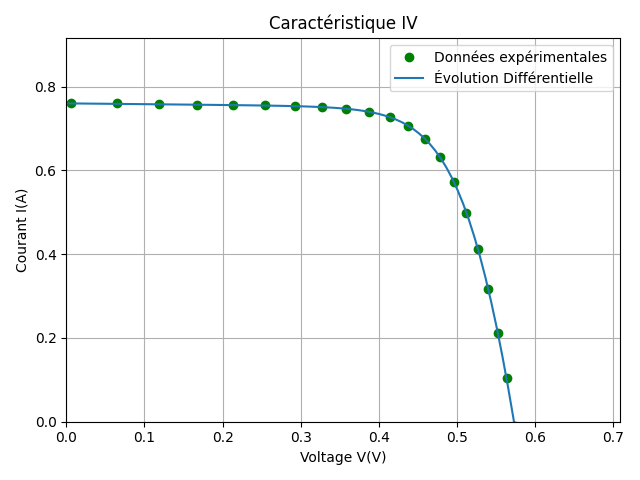
\includegraphics[width=\textwidth]{resources/RTCFrance/singled/iv.png}
        \caption{Comparaison entre la courbe expérimentale et la caractéristique calculée.}
    \end{subfigure}
    ~
    \begin{subfigure}[b]{0.45\textwidth}
        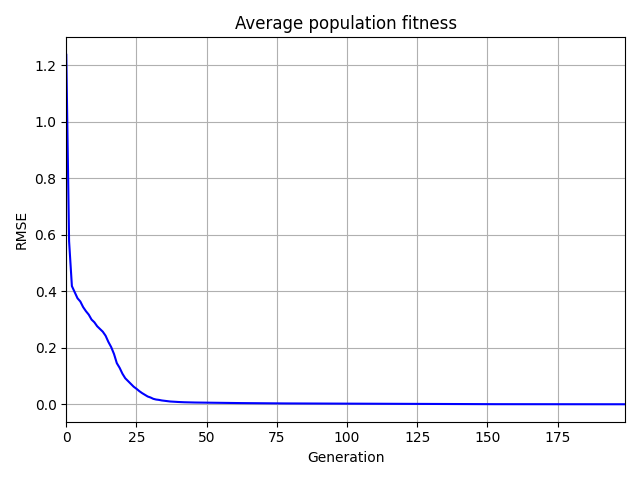
\includegraphics[width=\textwidth]{resources/RTCFrance/singled/fitness.png}
        \caption{Évolution de la valeur moyenne de fitness de chaque génération}
    \end{subfigure}
    \caption{Résultats de l'ED appliquée sur la cellule RTC France 57 mm.}
    \label{fig:RTCres}
\end{figure*}

\begin{table}
  \caption{Comparaison de l'ED avec d'autres méthodes dans la littérature}
  \label{tab:RTCres}

  \begin{center}
  \scriptsize
    \begin{tabular*}{\textwidth}{l@{\extracolsep{\fill}}cllllll }
       \hline
       Paramètres & Référence & $R_s$ (\si{\ohm}) & $R_{sh} (\si{\ohm})$ & $a $ & $I_0$ (\si{\micro\ampere}) & $I_{PV}$ (\si{\ampere}) & $RMSE$ \\
       \hline
       ED (simple diode) &                            & \num{0.0363} & \num{54.1134} & \num{1.4709} & \num{0.3209} & \num{0.7607} & \num{7.7692e-04}\\
       ED3P              & \cite{Chin2019}            & \num{0.0363} & \num{54.1924} & \num{1.4798} & \num{0.3191} & \num{0.7607} & \num{8.1291e-04}\\
       PSO               & \cite{Hamid2016}           & \num{0.0363} & \num{53.8550} & \num{1.4816} & \num{0.3245} & \num{0.7607} & \num{9.8606e-04}\\
       ABC               & \cite{Oliva2014}           & \num{0.0364} & \num{53.6433} & \num{1.4817} & \num{0.3251} & \num{0.7608} & \num{9.8620e-04}\\
       Newton            & \cite{Easwarakhanthan1986} & \num{0.0364} & \num{53.7634} & \num{1.4837} & \num{0.3223} & \num{0.7608} & \num{9.70e-03}  \\
       GA                & \cite{Oliva2014}           & \num{0.0299} & \num{42.3729} & \num{1.5751} & \num{0.8087} & \num{0.7619} & \num{1.90e-02}  \\
       \hline
    \end{tabular*}
  \end{center}
\end{table}

\nomenclature{$ED3P$}{Évolution différentielle à trois points}
\nomenclature{ABC}{Colonies d'abeilles artificielles (\textit{Artificial Bee Colony Optimization})}

\subsubsection{Modèle double diode}
En ce qui concerne le modèle double diode, les deux facteurs d'idéalité $a_1$ et $a_2$ ainsi que les courants de saturation $I_{01}$ et $I_{02}$ sont indépendants les uns les autres mais sont contraints dans les limites dans le tableau \ref{tab:doubledboundaries}. Les résultats de l'ED en double diode sont comparés avec ceux de quelques autres méthode dans le tableau \ref{tab:RTCresdouble}.
\begin{table}[H]
  \caption{Bornes de l'espace de recherche à 7 dimensions}
  \label{tab:doubledboundaries}

  \begin{center}
    \begin{tabular*}{.7\textwidth}{l@{\extracolsep{\fill}}cc}
      \hline
      \textbf{Paramètre} & \textbf{Borne inférieure} & \textbf{Borne Supérieure}\\
      \hline
      $R_s$    & 0 & 1 \\
      $R_{sh}$ & 2 & 100 \\
      $a_1$    & 1 & 2\\
      $a_2$    & 1 & 2\\
      $I_{01}$ & \num{1e-07} & \num{1e-04} \\
      $I_{02}$ & \num{1e-07} & \num{1e-04} \\
      $I_{PV}$ & 0 & 10\\
       \hline
    \end{tabular*}
  \end{center}
\end{table}

\begin{table}[H]
  \caption{Comparaison de l'ED avec d'autres méthodes dans la littérature}
  \label{tab:RTCresdouble}

  \begin{center}
  \scriptsize
    \begin{tabular*}{\textwidth}{l@{\extracolsep{\fill}}cllllllll}
       \hline
       Paramètres & Référence & $R_s$ (\si{\ohm}) & $R_{sh} (\si{\ohm})$ & $a_1$ & $a_2$ & $I_{01}$ (\si{\ampere}) & $I_{02}$ (\si{\ampere}) & $I_{PV}$ (\si{\ampere}) & $RMSE$ \\
       \hline
       ED (double diode) &                            & \num{0.02061}   & \num{51.9345} & \num{1.87579} & \num{1.43602} & \num{4.2322e-07} 
                                                      & \num{1.8726e-07}& \num{0.76055} & \num{7.63e-04}   \\
       PSO               & \cite{Jordehi2016}         & \num{0.05861}   & \num{18.2106} & \num{1.00012} & \num{1.00091} & \num{2.8601e-10} 
                                                      & \num{1e-12}     & \num{0.7633}  & \num{8.1646e-03} \\
       GSA               & \cite{Jordehi2017}         & \num{0.02914}   & \num{51.116}  & \num{1.6087}  & \num{1.62889} & \num{6.60621e-7} 
                                                      & \num{4.55149e-7}& \num{0.76886} & \num{5.91958e-03}\\
       ABC               & \cite{Oliva2014}           & \num{0.0364}    & \num{53.7804} & \num{1.4495} & \num{1.4885} & \num{4.07e-08}
                                                      & \num{2.874e-07} & \num{0.7608}  & \num{9.861e-04}\\
       \hline
    \end{tabular*}
  \end{center}
\end{table}

\nomenclature{GSA}{Gravitational Search Algorithm}

\subsection{Cas 2: Module monocristallin Schutten Solar STM6-40/36}

Nous nous concernons dans ce deuxième cas d'étude du module monocristallin Schutten Solar STM6-40/36 composé de 36 cellules ($156\si{\milli\meter}\times 156\si{\milli\meter}$) en série. Les données expérimentales ont été prises à une température de 51\si{\celsius}. Une comparaison des résultats de l'ED avec d'autres méthodes est présentée dans le tableau \ref{tab:stm6}. La correspondance de la caractéristique calculée par l'ED aux points experimentaux est démontrée graphiquement dans la figure \ref{fig:STM6res}. Malgré la distribution irrégulière des points, l'ED arrive a produire une solution précise. Sa précision et de même ordre de grandeur que ED3P \cite{Chin2019} mais elle est supérieure aux techniques des colonies des abeilles artificielles (ABC) \cite{Oliva2014}, de sa version améliorée par Oliva et al. (CIABC) \cite{Oliva2017a} et Chaotic Whale Optimization Algorithm (CWOA) \cite{Oliva2017}.

\begin{figure*}[t!]
    \centering
    \begin{subfigure}[b]{0.45\textwidth}
        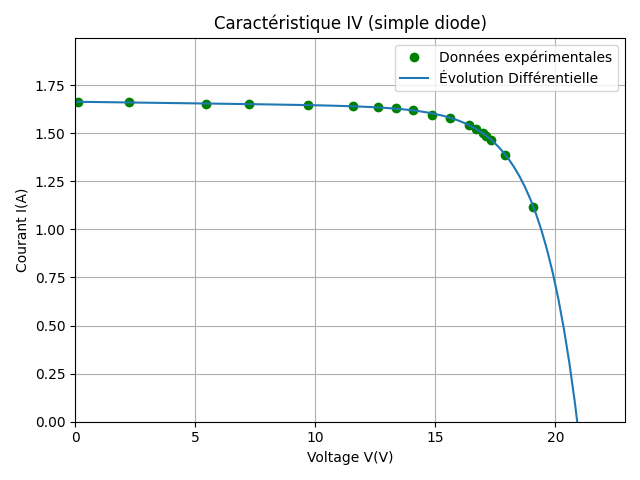
\includegraphics[width=\textwidth]{resources/STM6/singled/iv.png}
        \caption{Correspondence de l'ED aux données expérimentales. La distribution non-optimale des points n'entrave pas la convergence.}
    \end{subfigure}
    ~
    \begin{subfigure}[b]{0.45\textwidth}
        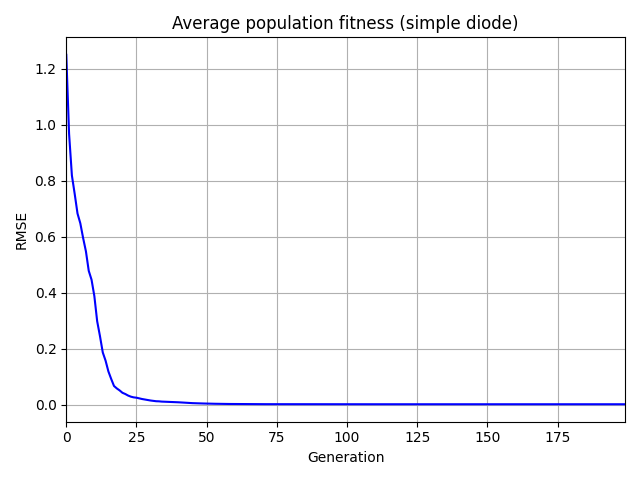
\includegraphics[width=\textwidth]{resources/STM6/singled/fitness.png}
        \caption{Évolution de la valeur moyenne de fitness de chaque génération. L'ED est convergeante dès la $50^{\text{ème}}$ itération.}
    \end{subfigure}
    \caption{Résultats de l'ED appliquée sur au module Schutten Solar STM6-40/36}
    \label{fig:STM6res}
\end{figure*}

\begin{table}
  \caption{Comparaison de l'ED avec d'autres méthodes dans la littérature sur le module STM6-40/36}
  \label{tab:stm6}

  \begin{center}
    \scriptsize
    \begin{tabular*}{\textwidth}{l@{\extracolsep{\fill}}cllllll}
      \hline
      Paramètres & Référence & $R_s$ (\si{\milli\ohm}) & $R_{sh} (\si{\ohm})$ & $a $ & $I_0$ (\si{\micro\ampere}) & $I_{PV}$ (\si{\ampere}) & $RMSE$ \\
      \hline
       ED (simple diode)  &                   & \num{0.2801} & \num{16.5854} & \num{1.5571} & \num{2.8049} & \num{1.6633} & \num{1.7721e-03}  \\
       ED3P               & \cite{Chin2019}   & \num{0.4186} & \num{16.7328} & \num{1.5656} & \num{2.7698} & \num{1.6632} & \num{1.7740e-03}  \\
       ABC                & \cite{Oliva2014}  & \num{4.99}   & \num{15.206}  & \num{1.4866} & \num{1.5}    & \num{1.6644} & \num{1.838e-03}   \\
       CIABC              & \cite{Oliva2017a} & \num{4.4}    & \num{15.617}  & \num{1.4976} & \num{1.6642} & \num{1.6760} & \num{1.819e-03}   \\
       CWOA               & \cite{Oliva2017}  & \num{5}      & \num{15.4}    & \num{1.5}    & \num{1.6338} & \num{1.7}    & \num{1.800e-03}   \\
       \hline
    \end{tabular*}
  \end{center}
\end{table}
\nomenclature{CIABC}{Chaotic Improved Artificial Bee Colony}
\nomenclature{CWOA}{Chaotic Whale Optimization Algorithm}

\subsubsection{Modèle double diode}

Les résultats de l'ED avec le modèle double diode sur le module STM6-40/36 sont présenté dans le tableau \ref{tab:STM6double} avec d'autres techniques tel quel les colonies d'abeilles artificielles et les essaims particulaires. Le tableau \ref{tab:stm6doublelimits} montre les bornes utilisées comme limites de l'espace de recherche. Notons la similarité des qualités des résultats du modèle simple et double diode.

\begin{table}[H]
  \caption{Comparaison de l'ED avec d'autres méthodes sur le module photovoltaïque STM6-40/36}
  \label{tab:STM6double}

  \begin{center}
  \scriptsize
    \begin{tabular*}{\textwidth}{l@{\extracolsep{\fill}}cllllllll}
       \hline
       Paramètres & Référence & $R_s$ (\si{\ohm}) & $R_{sh} (\si{\ohm})$ & $a_1$ & $a_2$ & $I_{01}$ (\si{\ampere}) & $I_{02}$ (\si{\ampere}) & $I_{PV}$ (\si{\ampere}) & $RMSE$ \\
       \hline
       ED (double diode) &                            & \num{0.0177}    & \num{16.7050}& \num{1.9049} & \num{1.52461}   & \num{1.006e-06} 
                                                      & \num{2.9858e-06}& \num{1.6633} & \num{1.7724e-03}   \\
       ELPSO             & \cite{RezaeeJordehi2018}   & \num{0.0138}    & \num{16.8580}& \num{1.8706} & \num{1.16648}   & \num{1.670e-08} 
                                                      & \num{6.21092e-6}& \num{1.6648} & \num{1.8307e-03}   \\
       ABC               & \cite{RezaeeJordehi2018}   & \num{0.03434}   & \num{26.0613}& \num{1.9851}  & \num{1.4687}** & \num{8.938e-6} 
                                                      & \num{1e-12}     & \num{1.66347}& \num{2.0538e-03}\\
       \hline
    \end{tabular*}
  \end{center}
\end{table}
\nomenclature{ELPSO}{Enhanced Leader Particle Swarm Optimization}

\begin{table}[H]
  \caption{Limites de l'espace de recherche pour l'ED double diode sur le module photovoltaïque STM6-40/36}
  \label{tab:stm6doublelimits}

  \begin{center}
    \begin{tabular*}{.7\textwidth}{l@{\extracolsep{\fill}}cc}
      \hline
      \textbf{Paramètre} & \textbf{Borne inférieure} & \textbf{Borne Supérieure}\\
      \hline
      $R_s$    & 0 & 1 \\
      $R_{sh}$ & 2 & 100 \\
      $a_1$    & 1 & 2\\
      $a_2$    & 1 & 2\\
      $I_{01}$ & \num{0} & \num{1e-04} \\
      $I_{02}$ & \num{0} & \num{1e-04} \\
      $I_{PV}$ & 0 & 10\\
      \hline
    \end{tabular*}
  \end{center}
\end{table}

\subsection{Analyse et cohérence de l'ED}

La performance supérieure démontrée par l'ED par rapport aux autres algorithmes provient probablement de ses capacités à la \textit{recherche globale}. L'existence d'une multitude de minimums locaux est demontrée dans la figure \ref{fig:neigh} où on a projeté l'espace de recherche 5-dimensionnel sur 2 dimensions au voisinage du minimum global. On fait varier le facteur d'idéalité $a$ et la résistance série $R_s$ dont le modèle est très sensible aux variations. Les trois autres paramètres $R_{sh}$, $I_0$ et $I_{PV}$ sont fixés sur les valeurs du minimum global retrouvé par l'ED comme dans le tableau \ref{tab:RTCres}.

\begin{figure}[H]
  \begin{center}
    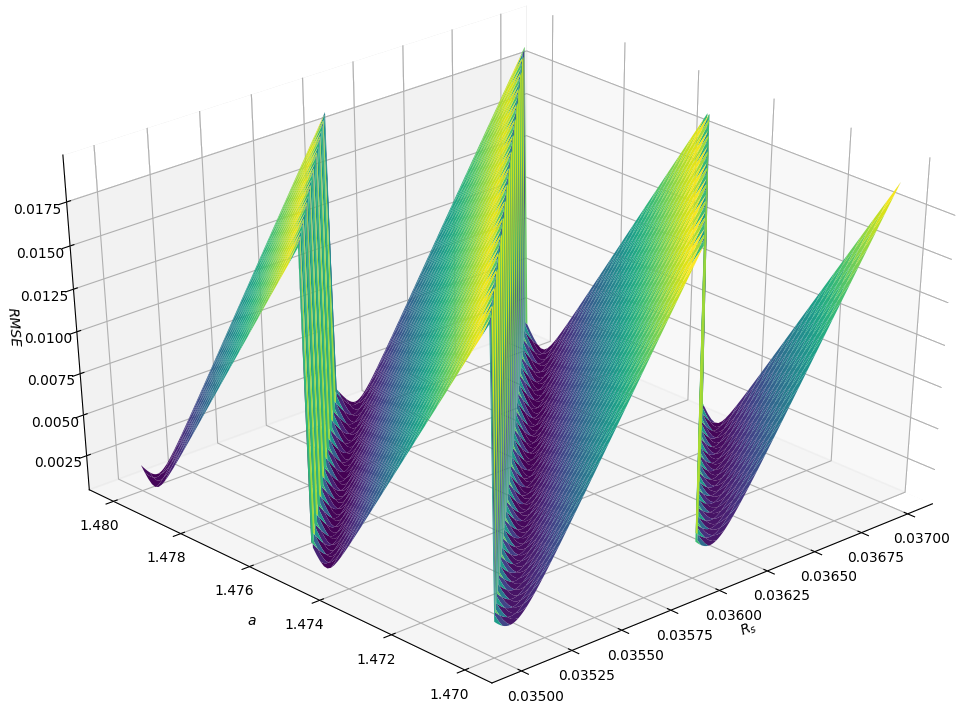
\includegraphics[width=0.5\textwidth]{resources/RTCFrance/singled/neighborhood.png}
    \caption{Le voisinage du minimum global retrouvé par l'ED selon le facteur d'idéalité et la résistance en série. Notons l'existence des "vallées" qui comprennent potentiellement plusieurs minimums locaux}
    \label{fig:neigh}
  \end{center}
\end{figure}

La nature stochastique de l'Évolution Différentielle fait qu'elle donne des résultats différents après chaque essai. Ceci impose une analyse de cohérence de la méthode pour estimer la fiabilité de l'ED pendant plusieurs essais consécutifs. Figure \ref{fig:consist} montre la RMSE de la solution finale dans 30 essais indépendants de l'ED.
Tous les points sont localisés dans une région très concentrée de l'espace de recherche ce qui indique que l'ED parvient effectivement à localiser le minimum global.
Les écart-types des paramètres montrés sur le tableau \ref{tab:RTCstats} confirment ceci puisque ils peuvent être interprétés comme un indice de "stabilité" de l'algorithme qui quantifié sa capacité a reproduire les mêmes résultats. Tous les écart-types sont de l'ordre de $10^{-3}$ ou moins, donc une solution précise est garantie dans n'importe quel essai.

\begin{figure}
    \begin{center}
      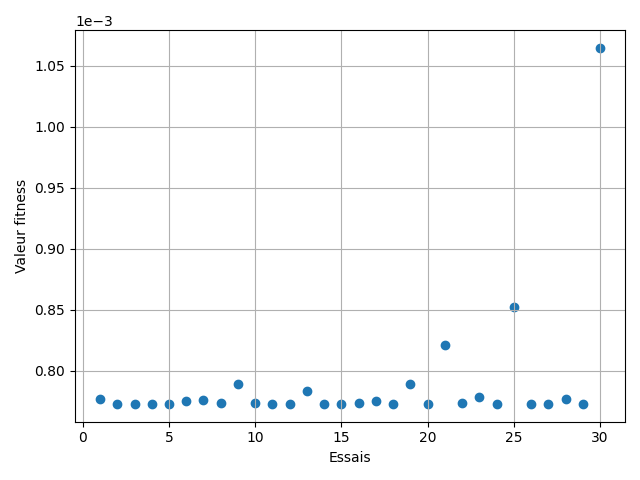
\includegraphics[width=.5\textwidth]{resources/RTCFrance/singled/consist.png}
      \caption{Les RMSEs obtenues lors de 30 essais indépendants sur la cellule RTC France 57 mm}
      \label{fig:consist}
    \end{center}
  \end{figure} 

\begin{table}
  \caption{Valeurs Moyennes de quelques paramètres influents de la cellule RTC France 57 mm et les écart-types associés des 30 essais}
  \label{tab:RTCstats}

  \begin{center}
    \begin{tabular*}{.7\textwidth}{c@{\extracolsep{\fill}}cc}
       \hline
       Paramètre & Valeur Moyenne & Écart-Type\\
       \hline
       $RMSE$       & \num{7.8925e-04}       & \num{5.3670e-05} \\
       $R_s$        & \num{3.6355e-02}       & \num{3.8936e-04} \\
       $a$          & \num{1.4722}           & \num{5.7539e-03} \\
       $I_0$        & \num{3.2655e-07}       & \num{3.4071e-08} \\
       \hline
    \end{tabular*}
  \end{center}
\end{table}

\section{Utilisation de l'outil \textit{DEPV}}

\section{Conclusion}

Le modèle double diode contient deux termes exponentiels nécessitant deux évaluations de la fonction W de Lambert pour chaque point expérimental, ce qui est relativement coûteux d'un point de vue de calcul numérique. Par ailleurs, puisque tous les parametres sont traités indépendamment des autres, l'espace de recherche est effectivement à 7 dimensions. Puisque la qualité des résultats des modèles simple et double diode est quasi-identique dans le cas de la cellule RTC France (Tableaux \ref{tab:RTCres} et \ref{tab:RTCresdouble} respectivement) ainsi que pour le module photovoltaïque monocristallin Schutten Solar STM6-40/36 (Tableaux \ref{tab:stm6} et \ref{tab:STM6double}), on constate que le modèle simple diode et très adéquat en terme de précision et supérieur en terme d'efficacité et rapidité de calcul.
